
\section{Class Introduction}
\subsection{Outline}

\begin{frame}
  \centering
  {\huge
    Week 1 -- Part 1: Class Introduction
  }
\end{frame}

\begin{frame}
  \frametitle{Outline}
  \begin{enumerate}
    \item Class Summary
    \item What are programming Challenges?
    \item Initial Example
    \item Class Program
    \item Lecturer Introduction
    \item Extra: ICPC
  \end{enumerate}
\end{frame}

\subsection{Class Summary}
\begin{frame}{Part I: Class Summary}
  \begin{itemize}
    \item In this class, you will \structure{practice your algorithm skills by writing many programs};
    \bigskip

    \item \structure{Key Idea:} Solve challenges with programs
    \begin{itemize}
      \item Read the problem and choose the right algorithm;
      \item Choose the implementation and data structure;
      \item Run the program and check the correct result;
    \end{itemize}
    \medskip

    \item In the 1st and 2nd year, we learn the \structure{theory} of many algorithm. In this lecture, we learn the \structure{practice} of these algorithms.
  \end{itemize}
\end{frame}

\begin{frame}{Algorithms: Theory x Implementation}
  \begin{exampleblock}{}
  It is very different to implement an algorithm in the classroom, and to implement an algorithm to solve a problem:
  \end{exampleblock}
  \begin{itemize}
    \item \structure{Data Structure}: You need to implement the function to read the input and store it in a data structure;
    \item \structure{Special Cases}: Special cases in the input can cause bugs or make the problem more complex;
    \item \structure{Large Input}: If the input is very large, the implementation
    needs to be efficient, or the program will run forever;
    \item \structure{Debugging}: It can be hard to debug if the input is very hard, you need to learn how to make a \structure{test input};
  \end{itemize}
\end{frame}

\begin{frame}{Automated Judging}
  \begin{exampleblock}{}
  In this lecture we use {\bf Automated Judges (AJ)} to check if your homework is correct.
  \end{exampleblock}

  \begin{itemize}
    \item An AJ is a website that proposes programming puzzles, and receive solutions;
    \begin{itemize}
      \item Ex: AtCoder, Aizu Online Judge, Topcoder, Codeforces, etc.
    \end{itemize}\bigskip

    \item The AJ receives your program; compile it; and grade it;\bigskip

    \item The AJ test your program with a set of \structure{Hidden Inputs}\bigskip

    \item The AJ gives you the result: \structure{Correct} or \alert{Incorrect}
    \begin{itemize}
      \item If the result is incorrect, it will not tell you why;
      \item You have to create debug cases by yourself;
      \item But, you can submit a new version as many times as you want;
    \end{itemize}
  \end{itemize}
\end{frame}

\begin{frame}{What this class expects of you}
  \begin{exampleblock}{Estimated classwork:}
    \begin{itemize}
      \item You need basic programming knowledge in C++;
      \medskip

      \item Complete 2-4 program assignments per week;
      \begin{itemize}
        \item Average of 4 hours of study per week;
        \item A lot of time with debug and creating test cases;
        \item (Atcoder difficulty: 300 to 500)
      \end{itemize}
      \medskip

      \item Homework starts easy, but becomes harder later in the course;
      \medskip

      \item No final exam: only assignments!
    \end{itemize}
  \end{exampleblock}
  \hfill {\bf Hint: Do your homework early!}
\end{frame}

\subsection{What are Programming Challenges?}
\begin{frame}{What kind of problem is a "Programming Challenge?"}
  A "Programming Challenge" gives you a problem, and you have to write a program to find the solution. Think of it as a {\bf programming puzzle}:

  \begin{block}{Simple Example}
    You want to schedule a pair dance club. Your friends give you their possible dates and times (Fri 14:00-15:00). What time do you choose to make the maximum number of pairs?
  \end{block}
  \bigskip

  \begin{itemize}
    \item Usually Programming challenges have a "story";
    \item There is a maximum execution time, so you have to use an efficient algorithm;
    \item Sometimes there are special cases;
    \item In general, a small program (< 200 lines) can solve the challenge;
  \end{itemize}
\end{frame}


\begin{frame}{Why programming challenges?}
  \begin{itemize}
    \item {\bf For Competitions}: Around 1980, Programming Contests started as a way for Computer Sciences universities to compete. (IOI, ICPC, etc)
    \bigskip

    \item {\bf For Study}: After 2000, many people use online Automated Judges to study programming and prove their ability; (TopCoder, Codeforces, AtCoder, etc);
    \bigskip

    \item {\bf For Recruitment}: Recently, many companies use Programming Challenges to test the programming ability of candidates. candidates. (Google, Facebook, etc)\bigskip

    \item {\bf For Fun}: Some people just like to have an excuse to program!
  \end{itemize}
\end{frame}

\subsection{Example}
\begin{frame}{Real Example (from homework): The 3n+1 problem}
  \begin{columns}
    \column{0.55\textwidth}
      Contents of a Programming Challenge:
      \begin{itemize}
        \item Problem Description;
        \item Input Description;
        \item Output Description;
        \item Input/Output Example;
      \end{itemize}

    \column{0.45\textwidth}
    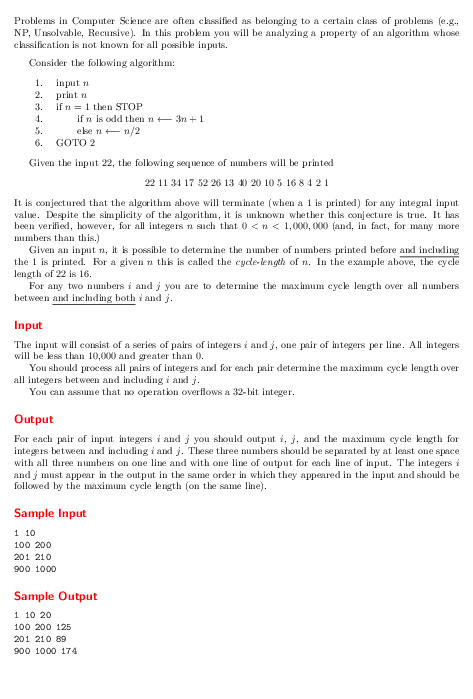
\includegraphics[width=1\textwidth]{img/3n_problem}
  \end{columns}
\end{frame}

\begin{frame}{Real Example (from homework): The 3n+1 problem}{How to solve?}
  \begin{columns}
    \column{0.55\textwidth}
    {\smaller
    The problem wants the \structure{longest sequence size} generated by the following algorithm:
      \begin{enumerate}
        \item if $n = 1$ then STOP
        \item if $n$ is odd, then $n = 3n + 1$
        \item else $n = n/2$
        \item GOTO 1
      \end{enumerate}
    \medskip

    For example, if $i = 1$ and $j = 4$:
    \begin{itemize}
      \item n = 1: 1 END; {\bf Length 1}
      \item n = 2: 2 1 END; {\bf Length 2}
      \item n = 3: 3 10 5 16 8 4 2 1 END; {\bf Length 8}
      \item n = 4: 4 2 1 END; {\bf Length 3}
    \end{itemize}
    So the {\bf maximum length} is 8 (for n = 3)}
    \column{0.45\textwidth}
    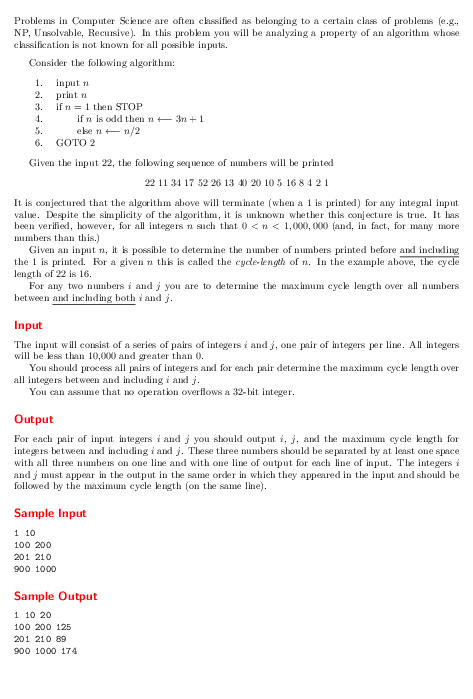
\includegraphics[width=1\textwidth]{img/3n_problem}
  \end{columns}
\end{frame}

\begin{frame}[fragile]{Real Example (from homework): The 3n+1 problem}{A simple program}
{\smaller
\begin{verbatim}
int main() {
  int min, max;
  int maxcycle = 0;
  cin >> min >> max;
  for (int i = min; i <= max; i++) {
    int cycle = 1;
    int n = i;
    while (n != 1) {
      if (n % 2 == 0) { n = n / 2; }
      else { n = n*3 + 1; }
      cycle++;
    }
    if (cycle > maxcycle) maxcycle = cycle;
  }
  cout << min << " " << max << " " << maxcycle << "\n";
  return 0;
}
\end{verbatim}}
\end{frame}

\begin{frame}{Real Example (from homework): The 3n+1 problem}{Simple programs, simple
  problems}

The solution in the last slide has some problems. One problem is that
it can be very slow! Consider the following case:
\bigskip

i = 1, j = 10:
\begin{itemize}
  \item n = 1: 1 END
  \item n = 2: 2 1 END
  ...
  \item n = 7: 7 22 11 34 17 52 26 13 40 20 10 5 16 8 4 2 1 END\\
  ...
  \item n = 9: 9 28 14 \alert{7 22 11 34 17 52 26 13 40 20 10 5 16 8 4 2 1 END}
  \item n = 10: \alert{10 5 16 8 4 2 1 END}
\end{itemize}
\bigskip

A lot of work is repeated without necessity. How to make the program faster?
\end{frame}

\begin{frame}{Real Example (from homework): The 3n+1 problem}{Memoization}
  A technique called {\bf Memoization} can solve the "repeated work" problem.
  \bigskip

  {\bf Memoization}:
  \begin{itemize}
    \item Every time you finish a calculation, store the result in the memory;
    \item Before you begin a calculation, check if it is not in the memory;
  \end{itemize}
  \bigskip

  This technique can reduce the amount of repeated work.
  \bigskip

  In this course we will review and study many techniques like this one. You will have to implement these techniques in the homework to make it efficient.
\end{frame}

\subsection{Class Program}
\begin{frame}{Topics in this class}
  \begin{enumerate}
    \item Introduction Problems
    \item Data Structures
    \item Search Problems
    \item Dynamic Programming
    \item Graphs Problems (Graph Structure)
    \item Graph Problems (Graph Search and Flow)
    \item String Manipulation
    \item Math Problems
    \item Geometry Problems
    \item Final Remix
  \end{enumerate}
\end{frame}

\begin{frame}{Class Format}
  \begin{block}{Weekly Schedule}
    \begin{itemize}
      \item Lecture Notes and Videos: Explanation about algorithms;
      \item TEAMS meeting with instructor to ask questions;
      \item Solve the homework at URI Online Judge;
    \end{itemize}
  \end{block}

  \begin{exampleblock}{Evaluation}
    \begin{itemize}
      \item No final examination;
      \item Grade based on number of homework completed every week;
    \end{itemize}
  \end{exampleblock}
\end{frame}

\subsection{Lecturer Introduction}
\begin{frame}
  \frametitle{About the Lecturer}
  \begin{columns}
    \column{0.4\textwidth}
    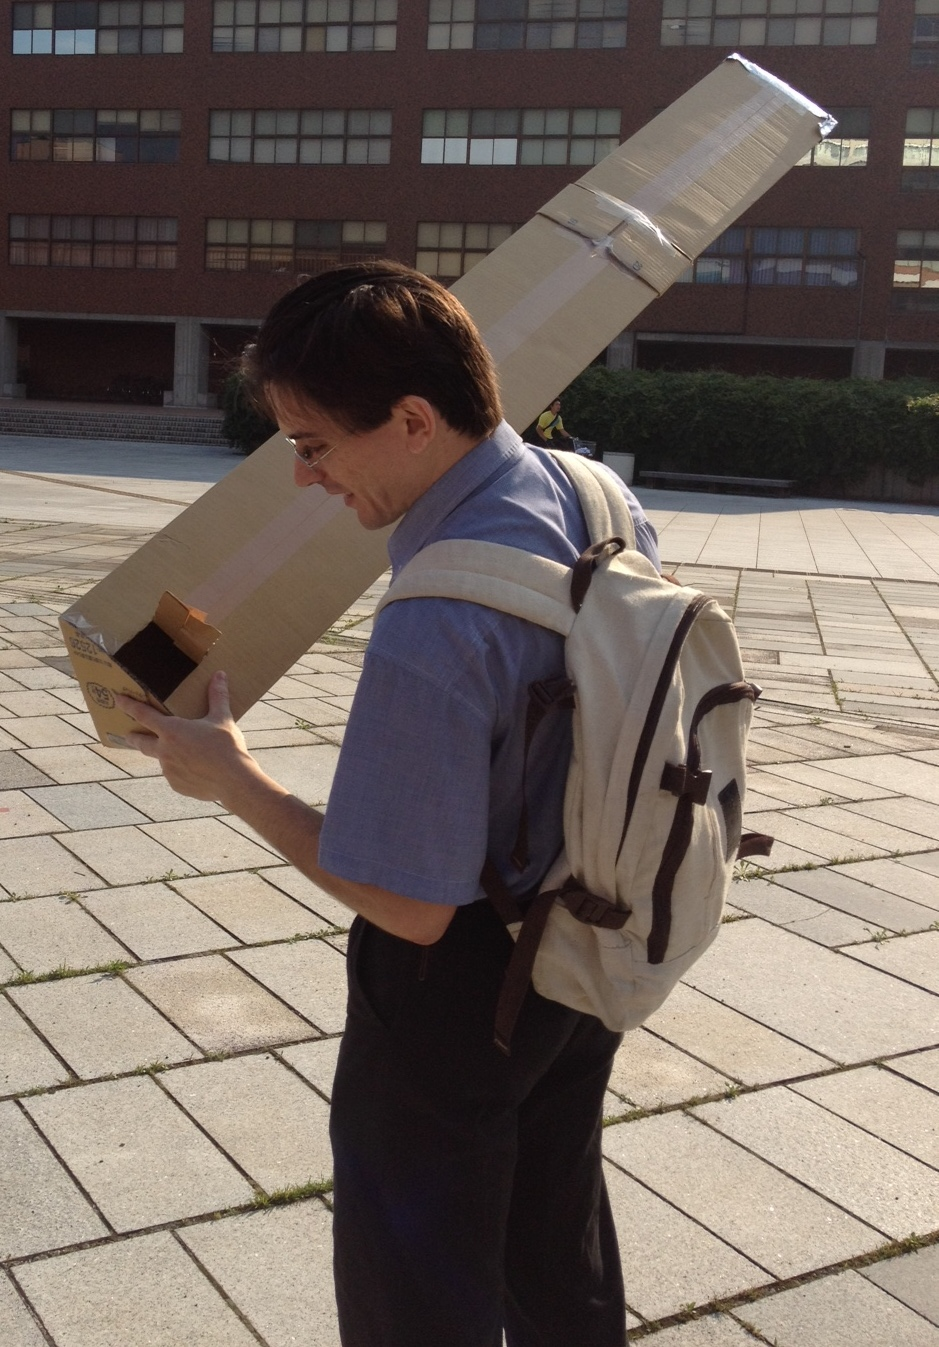
\includegraphics[height=.8\textheight]{../img/pinhole}
    \column{0.6\textwidth}
    {\small
    \begin{itemize}
      \item \structure{Name:} Claus Aranha;
      \item \structure{Country:} Brazil;
      \item \structure{Research Topics:}
      \begin{itemize}
        \item Evolutionary Computation;
        \item Artificial Life;
      \end{itemize}
      \item \structure{Hobbies:}
      \begin{itemize}
        \item Game Programming;
        \item Geocaching;
      \end{itemize}
        \medskip

      \item \structure{webpage:}\\ {\smaller \url{http://conclave.cs.tsukuba.ac.jp}}
    \end{itemize}
    }
  \end{columns}
\end{frame}

\subsection{ICPC}
\begin{frame}{Extra: Join the Tsukuba ICPC Team!}{What is ICPC?}
  \hfill 
\includegraphics[width=0.4\textwidth]{img/icpclogo}\\
  If you like these contests, and want an extra challenge, please consider
  joining the Tsukuba ICPC team!
  \bigskip

  ICPC (International Collegiate Programming Contest) is the largest and
  most traditional programming competition between universities.
  \bigskip

  More than 50.000 students from all over the world participate in this
  competition every year.
  \bigskip

  Contest Website: \url{https://icpc.baylor.edu/}
\end{frame}

\begin{frame}{Extra: Join the Tsukuba ICPC Team!}{Program and see the world!}
  \hfill 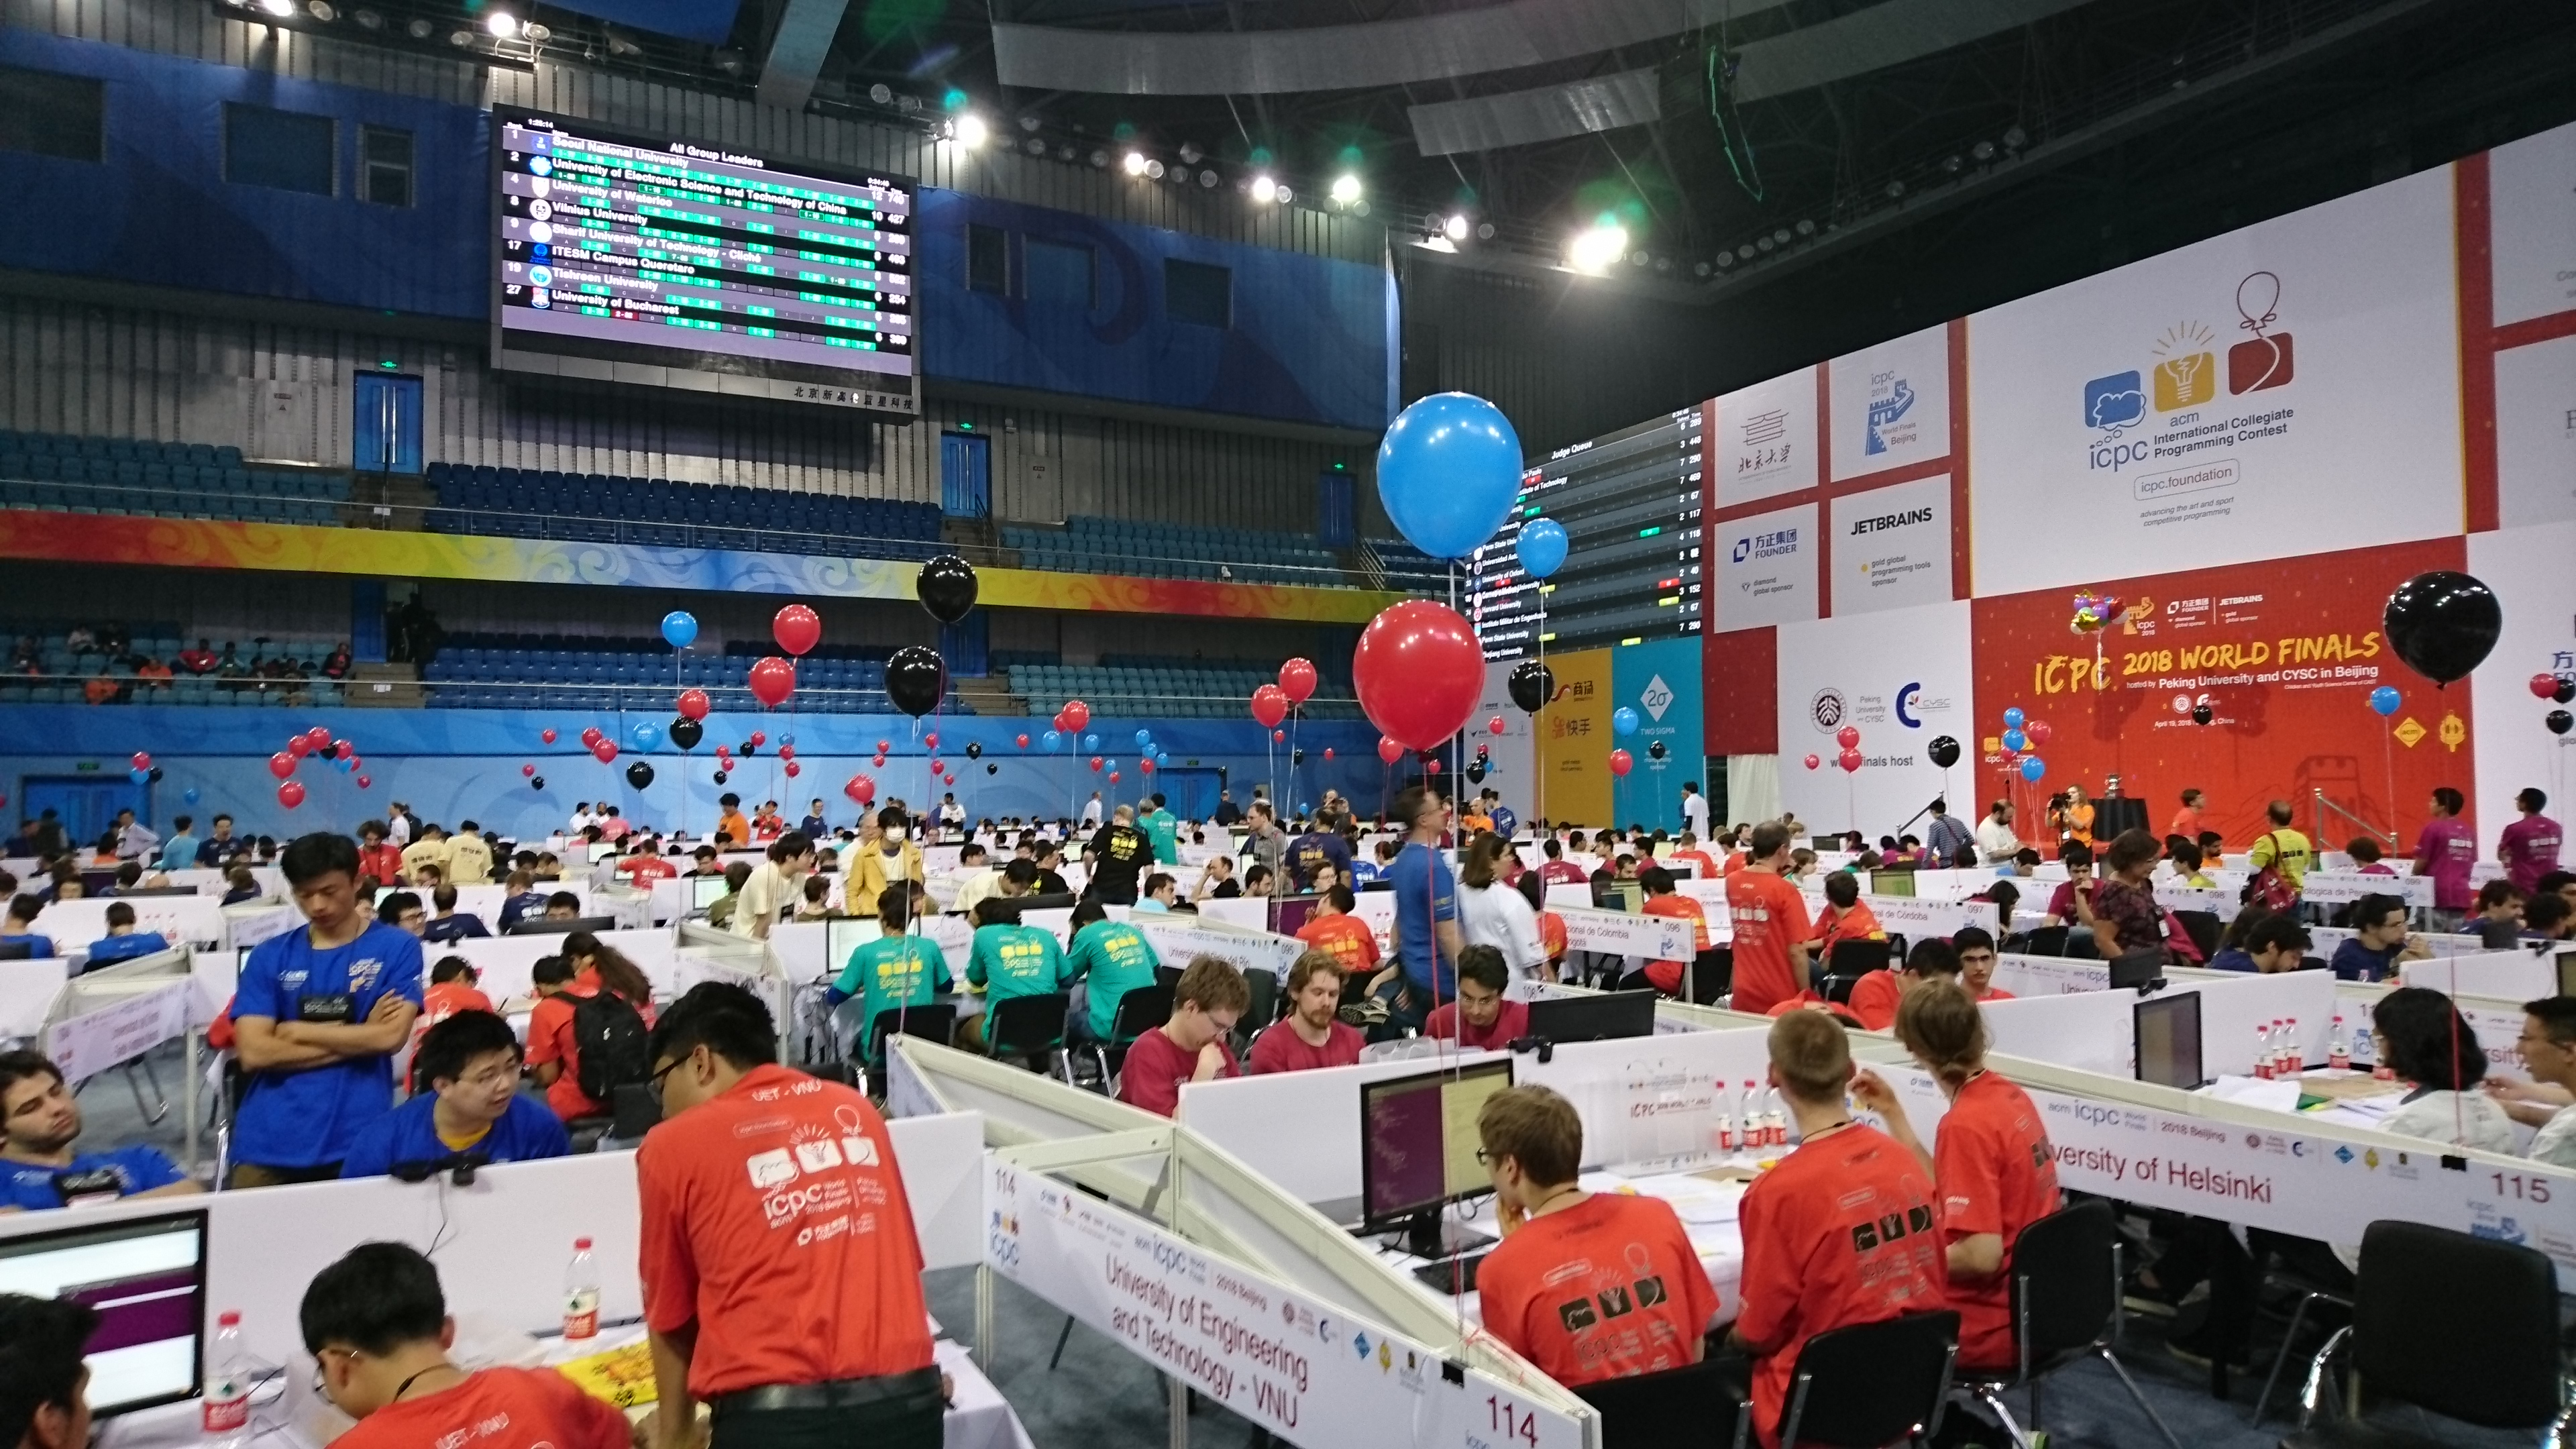
\includegraphics[width=0.4\textwidth]{img/icpc_image1}
  \begin{itemize}
    \item \alert{Requirements}: Team of 3 students, any course;
    \medskip

    \item \alert{Schedule:}
    \begin{itemize}
      \item National Preliminary Competition in July
      \item Japanese Regional Competition in October
      \item Asian Semi-final in December
      \item World Final April next year
    \end{itemize}
      (\alert{Dates may change this year because of nCov-19})
    \medskip
    \item Contact me if you're interested!
  \end{itemize}
\end{frame}



%%%%%%%%%%%%%%%%%%%%%%%%%%%%%%%%%%%%%%%%%%%%%%%%%%%%%%%%%%%%%%%%%%%%%%%%%%%%
